\chapter{Servidor}

O servidor é o software embarcado no HPS do Soc. Ele é o responsável por gerenciar a comunicação entre a interface de rede por onde recebe os dados provenientes do pacote ROS (cliente) e o FPGA\@.

A primeira etapa a ser concluída no desenvolvimento do servidor é compilação de uma versão linux para processadores ARM que será instalada no kit de desenvolvimento. O fluxo de boot do linux na placa é resumido na Figura~\ref{fig:linux}. 

\begin{figure}[ht]
	\caption{Boot linux embarcado}
	\begin{center}
		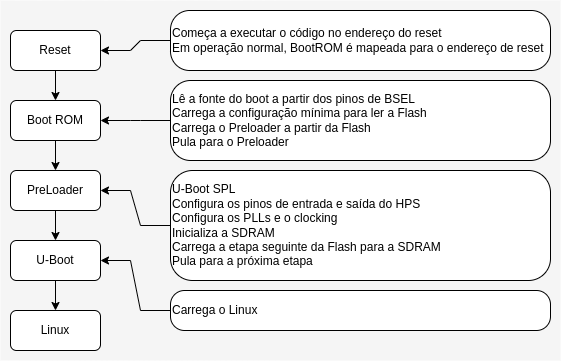
\includegraphics[scale=0.5]{imagens/embeddedLinux.png}\\
		{\small \textbf{Fonte:}\cite{SocLinux}}
    \end{center}\label{fig:linux}
\end{figure}

O primeiro elemento de software é o \textit{Boot ROM} que está gravado de fábrica internamente no dispositivo. Os arquivos de \textit{PreLoader},\textit{ U-boot} e do sistemas de aquivos do linux são salvos em um cartão de memória micro SD\@.

O \textit{Secondary Program Loader - SPL}, conhecido como \textit{PreLoader}, é executado a partir da Boot ROM\@. Ele é responsável por configurar o sistema para que o \textit{bootloader} (U-boot) possa ser executado. A Intel fornece uma ferramenta chamada BSP editor que, a partir de arquivos que descrevem o hardware, podem gerar o PreLoader para o projeto específico~\cite{SocLinux}.  

A etapa seguinte ao \textit{PreLoader} é o \textit{bootloader}. Nessa fase do boot todas as questões de baixo nível do SoC, como por exemplo, os clocks, pinos e SDRAM, já foram inicializados e estão prontos. O objetivo do bootloader, é obter essas informações do sistema e fazer com que ele funcione até o ponto onde o linux possa ser iniciado. Outra função importante do U-boot em um SoC Intel é programar o FPGA~\cite{SocLinux}. 

% Com todas as etapas do boot finalizadas o linux já estará sendo executado pelo HPS e pronto para o desenvolvimento do servidor. Os códigos do servidor podem ser baixados a partir do repositório disponível na referência \cite{interface-socket-server}. Após baixar a biblioteca de comunicação \cite{Pereira-Neto-Biblioteca} e executar sua compilação e instalação, os códigos do servidor poderão ser baixados e compilados. O Servidor mantém porta aberta para estabelecer uma conexão com o cliente e assim que a conexão é estabelecida, o cliente já pode começar a enviar os dados. Ao receber os dados do cliente, o servidor envia-os ao FPGA que os processa e os devolve ao servidor para que ele possa reenviar os dados já processados ao cliente. Um fluxograma simplificado desse processo pode ser visualizado na Figura \ref{fig:fluxoServidor}.

O acesso do servidor ao FPGA é feito através de mapeamento de endereços do linux, os SoCs Intel possuem uma arquitetura de memória mapeada. Para facilitar essa tarefa a Intel possui uma ferramenta chamada de \textit{sopc-create-header-files} integrada ao Quartus Prime (software de desenvolvimento para FPGAs Intel) que, através dos arquivos do projeto do sistema, consegue gerar um arquivo cabeçalho com todos os endereços para os periféricos relacionados ao FPGA\@. Portanto, o arquivo cabeçalho gerado disponibiliza o \textit{offset} do endereço em que cada periférico está localizado, assim, o servidor pode enviar e/ou receber dados ao periférico conhecendo o endereço da FPGA-bridge em que este periférico está conectado.

\begin{figure}[ht]
	\caption{Fluxograma simplificado do servidor}
	\begin{center}
		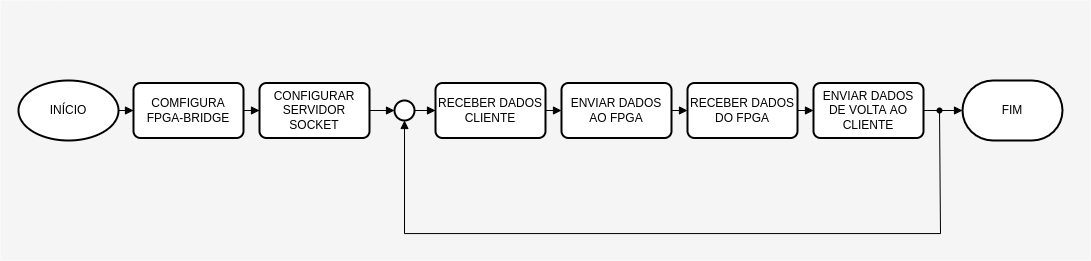
\includegraphics[scale=0.47]{imagens/fluxogramaServidor.png}\\
		{\small \textbf{Fonte:}Elaborado pelo autor}
    \end{center}\label{fig:fluxoServidor}
\end{figure} 
